%!TEX root = ../MasterThesis.tex

\section{Objectives of System}
\label{sec:system_objectives}

Based on the explanations in Chapter~\ref{cha:context_analysis}, and especially the scope definition for this Master thesis in Section~\ref{sec:scope_thesis}, the system for investigating E-commerce fraud incidents have to answer the central question:\@

\begin{quotation}
    \textit{Is this really a fraudulent E-commerce transaction?}
\end{quotation}

The main stakeholders, that need to be involved in the investigation process are:\@

\begin{itemize}
    \item the online merchants
    \item the \gls{PSP}
    \item the issuer
    \item the \gls{LSP}
\end{itemize}

Ideally they would make part of their internal information available for external partners to access and query for, so that the party, who has to authorize or validate the credit card payment can analyse all available information, as depicted in the Figure~\ref{fig:images_system_overview}.\@

\begin{figure}[H]
	\centering
		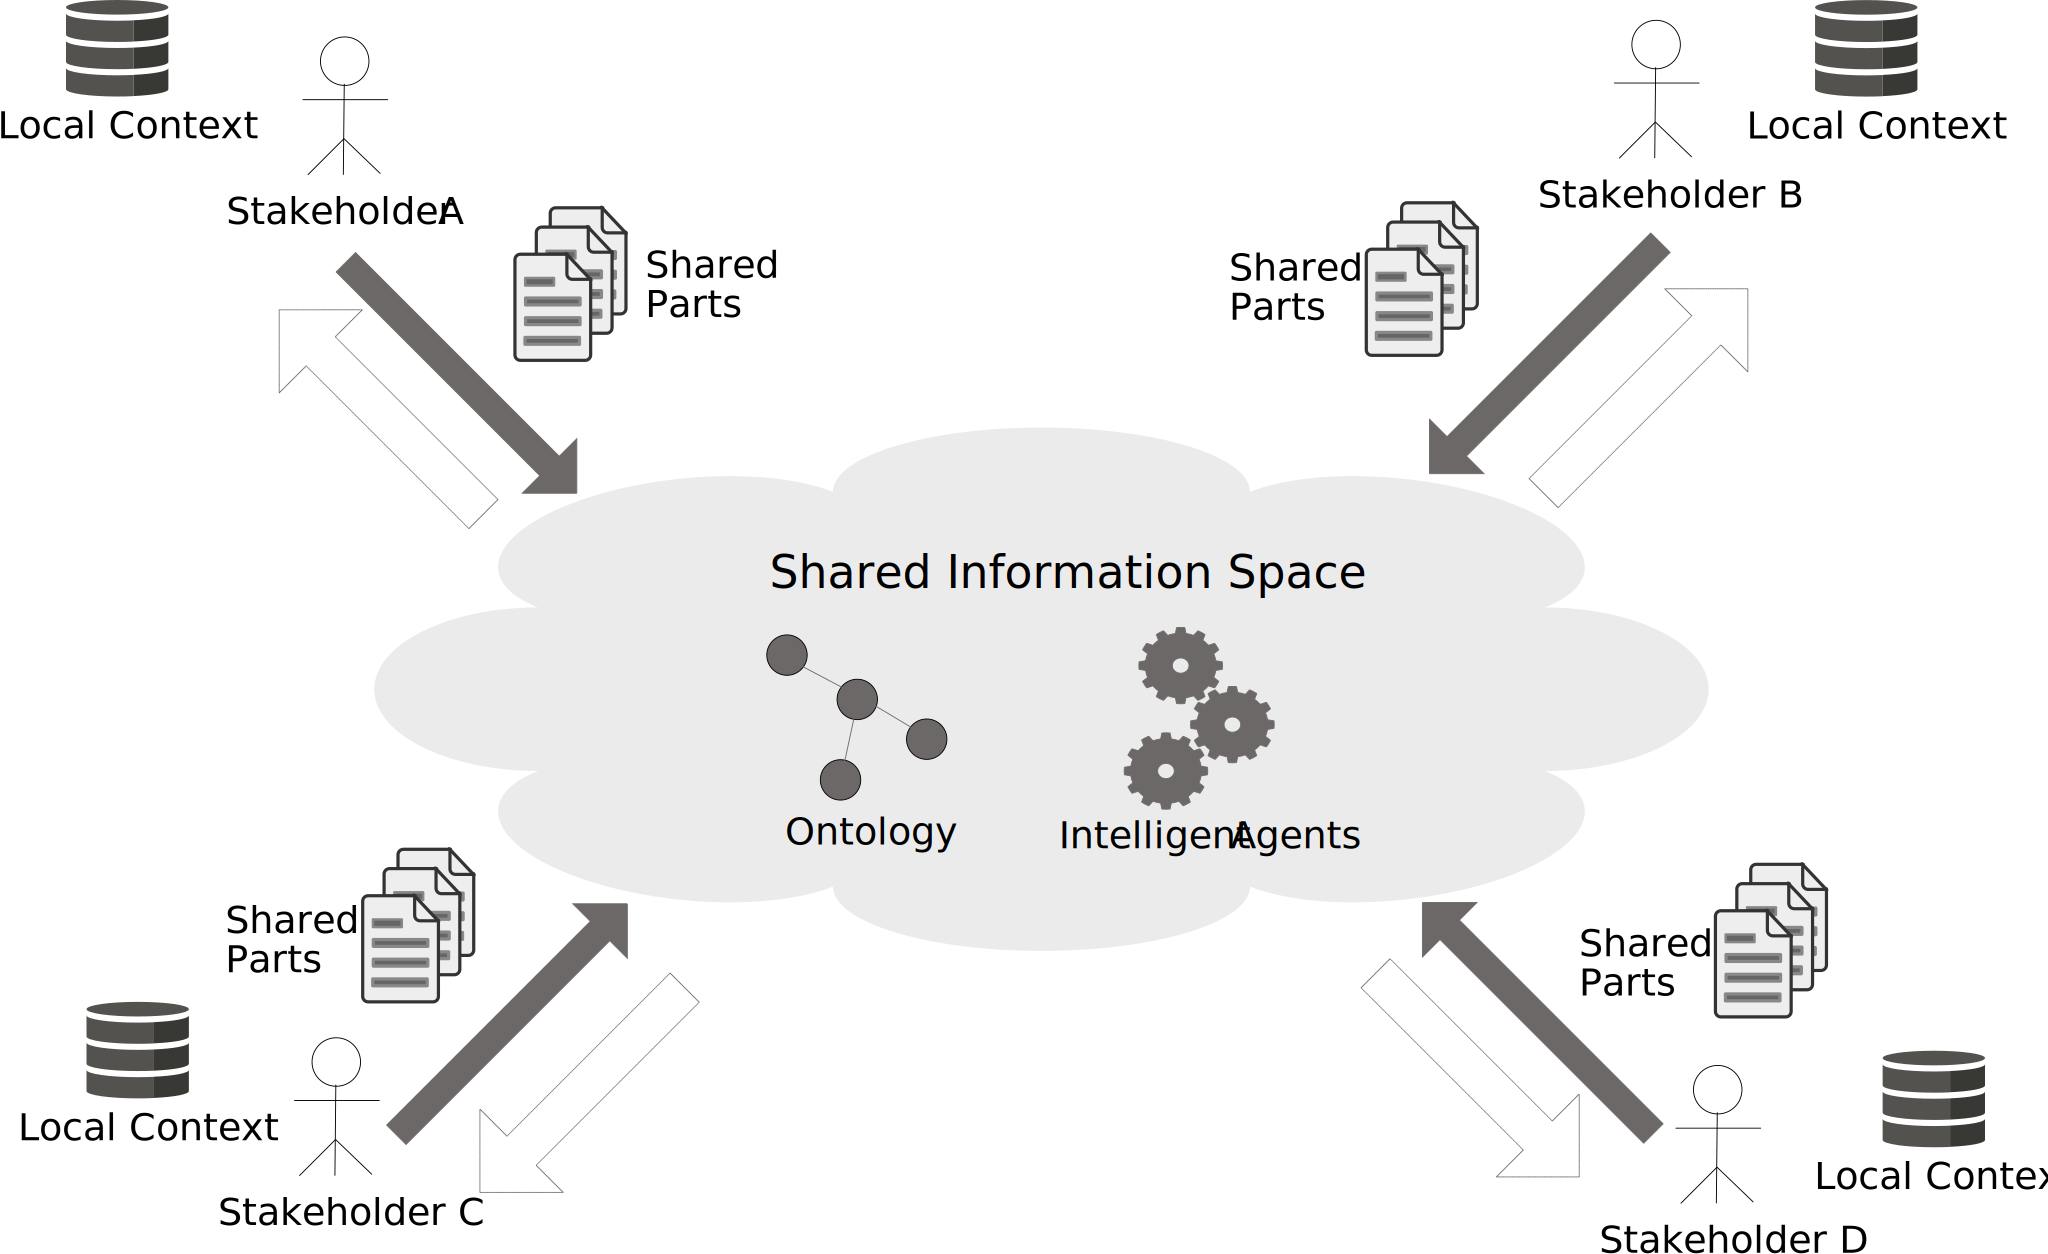
\includegraphics[width=0.8\columnwidth]{images/system_overview.pdf}
	\caption{System Overview}
\label{fig:images_system_overview}
\end{figure}

As the information is coming from various sources there has to be a shared data model that brings all of them together and defines the connection points and references for the parts of each stakeholder. Based on the discussion in Chapter~\ref{cha:context_analysis} and the analysis of the information each stakeholder has and transmit to others, the following initial schema can be conducted (see Figure~\ref{fig:images_data_model}).\@

\begin{figure}[H]
	\centering
		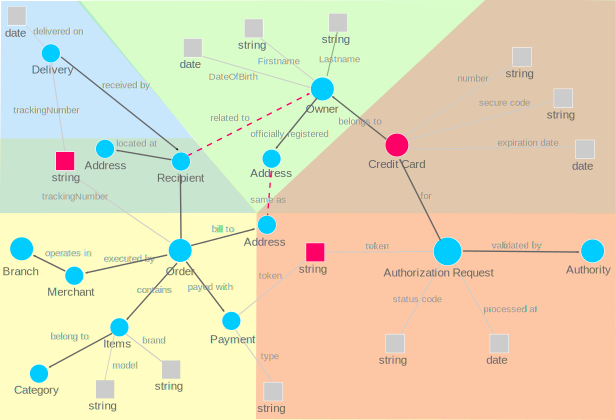
\includegraphics[width=0.8\columnwidth]{images/ontology_scenario_1.pdf}
	\caption{Initial Data Model}
\label{fig:images_data_model}
\end{figure}

\ldots

% section system_overview (end)
